\documentclass{standalone}
\usepackage{tikz}
\usetikzlibrary{patterns, positioning}
\usepackage[sfdefault]{ClearSans} %% option 'sfdefault' activates Clear Sans as the default text font
\usepackage[T1]{fontenc}

\begin{document}
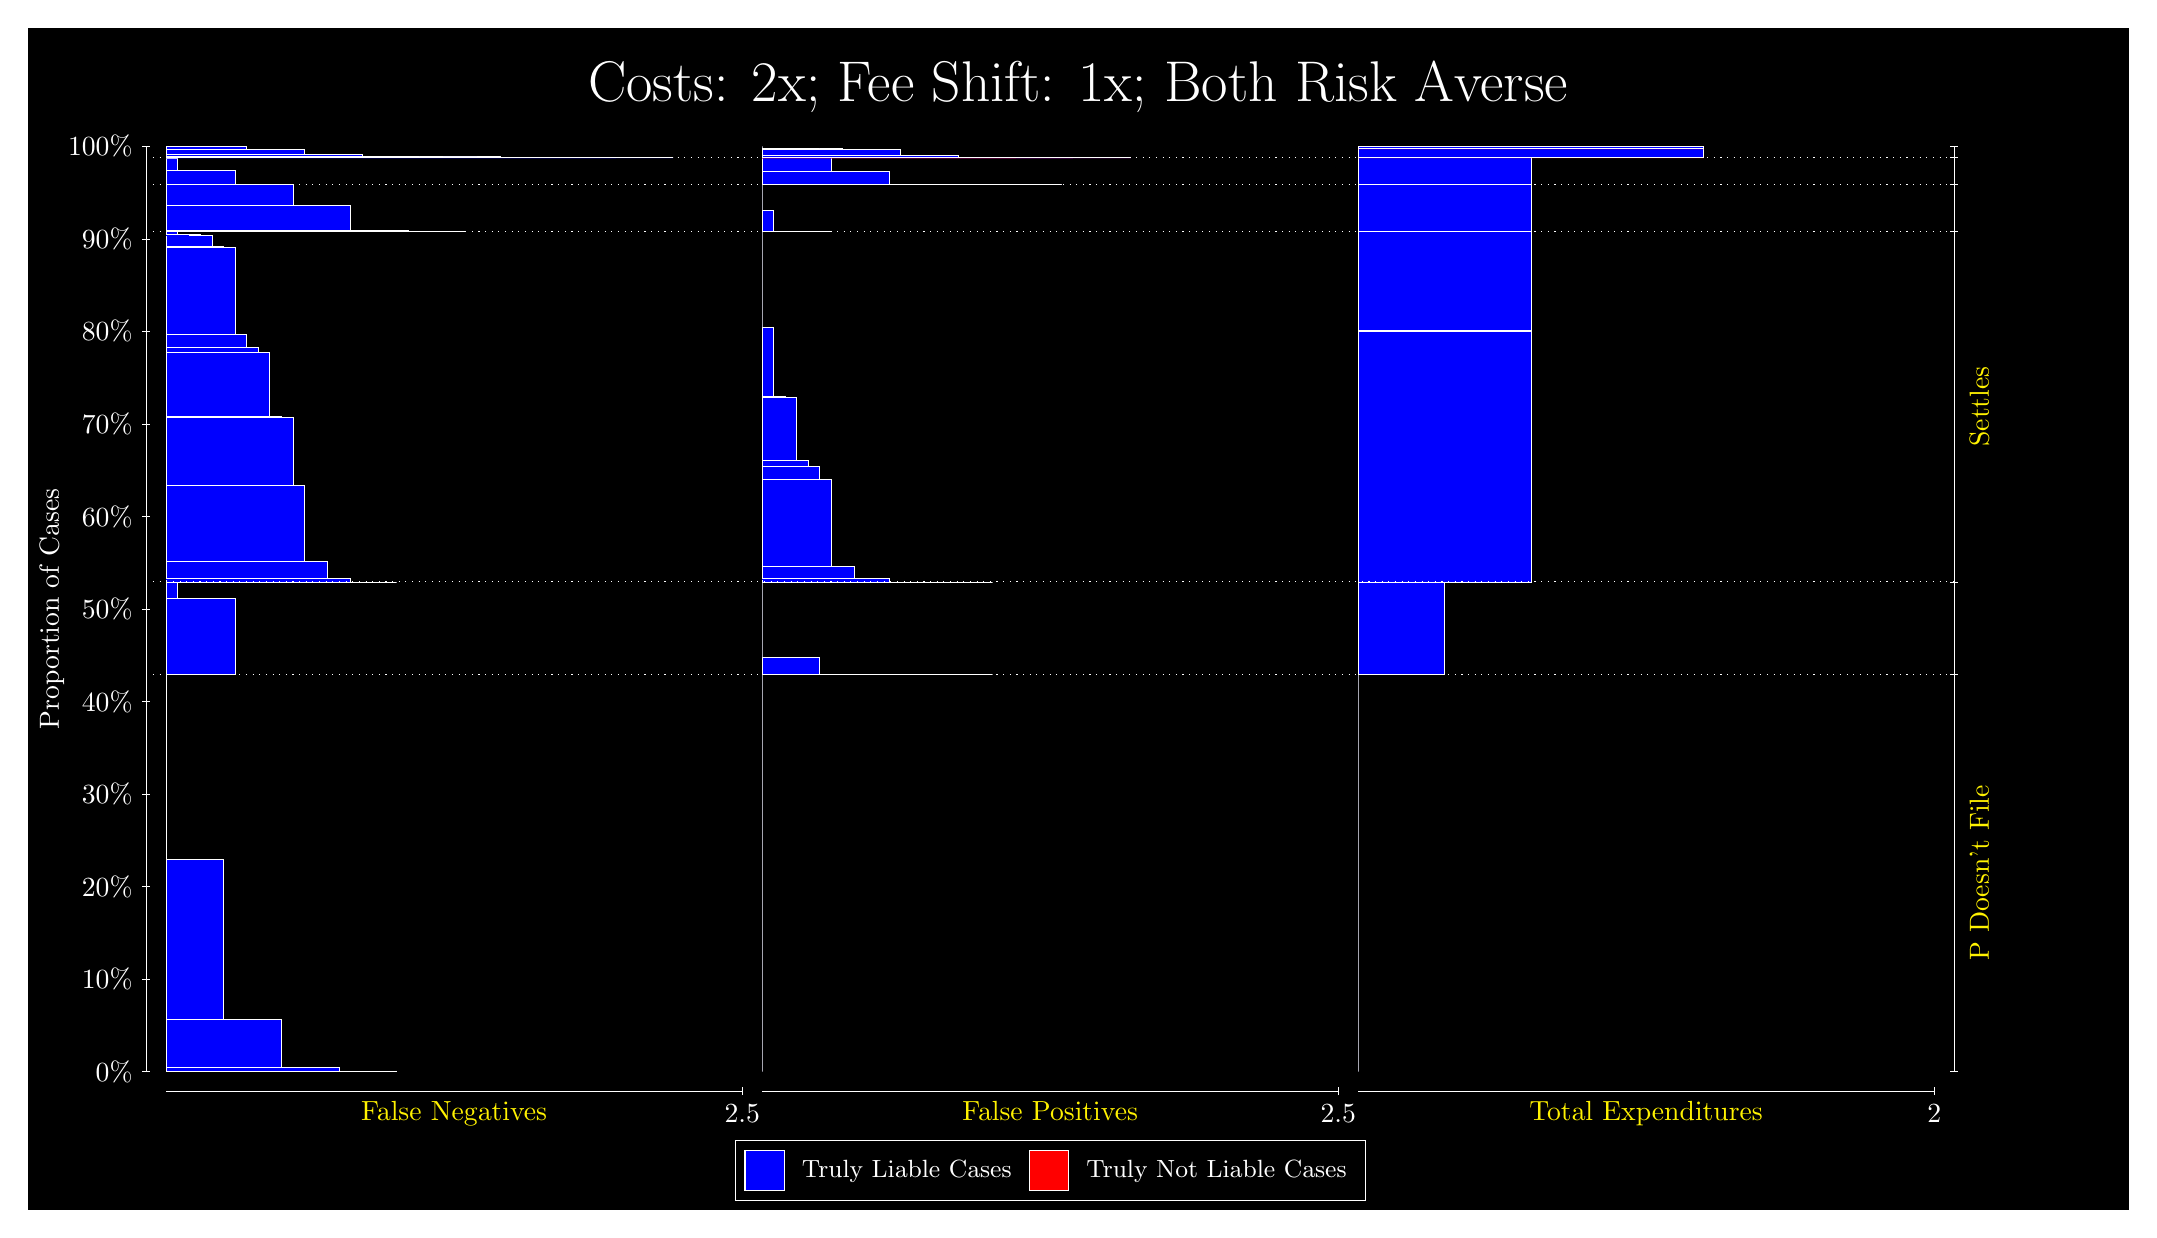
\begin{tikzpicture}
\draw[fill=black] (0,0) rectangle (26.667,15);
\draw[text=white] (0,13.5) rectangle (26.667,15) node[midway] {\huge Costs: 2x; Fee Shift: 1x; Both Risk Averse};
\draw[white, very thin] (1.5,1.75) -- (1.5,13.5);
\node[rotate=90, text=white, anchor=center] at (0.3, 7.625) {Proportion of Cases};
\draw[white, very thin] (1.45,1.75) -- (1.55,1.75);
\node[text=white, anchor=east] at (1.45, 1.75) {0\%};
\draw[white, very thin] (1.45,2.925) -- (1.55,2.925);
\node[text=white, anchor=east] at (1.45, 2.925) {10\%};
\draw[white, very thin] (1.45,4.1) -- (1.55,4.1);
\node[text=white, anchor=east] at (1.45, 4.1) {20\%};
\draw[white, very thin] (1.45,5.275) -- (1.55,5.275);
\node[text=white, anchor=east] at (1.45, 5.275) {30\%};
\draw[white, very thin] (1.45,6.45) -- (1.55,6.45);
\node[text=white, anchor=east] at (1.45, 6.45) {40\%};
\draw[white, very thin] (1.45,7.625) -- (1.55,7.625);
\node[text=white, anchor=east] at (1.45, 7.625) {50\%};
\draw[white, very thin] (1.45,8.8) -- (1.55,8.8);
\node[text=white, anchor=east] at (1.45, 8.8) {60\%};
\draw[white, very thin] (1.45,9.975) -- (1.55,9.975);
\node[text=white, anchor=east] at (1.45, 9.975) {70\%};
\draw[white, very thin] (1.45,11.15) -- (1.55,11.15);
\node[text=white, anchor=east] at (1.45, 11.15) {80\%};
\draw[white, very thin] (1.45,12.325) -- (1.55,12.325);
\node[text=white, anchor=east] at (1.45, 12.325) {90\%};
\draw[white, very thin] (1.45,13.5) -- (1.55,13.5);
\node[text=white, anchor=east] at (1.45, 13.5) {100\%};

\draw[white, very thin] (24.457,1.75) -- (24.457,13.5);
\draw[white, very thin] (24.407,1.75) -- (24.507,1.75);
\node[anchor=west] at (24.407, 1.75) {};
\draw[white, very thin] (24.407,6.7944) -- (24.507,6.7944);
\node[anchor=west] at (24.407, 6.7944) {};
\draw[white, very thin] (24.407,7.9686) -- (24.507,7.9686);
\node[anchor=west] at (24.407, 7.9686) {};
\draw[white, very thin] (24.407,12.422) -- (24.507,12.422);
\node[anchor=west] at (24.407, 12.422) {};
\draw[white, very thin] (24.407,13.018) -- (24.507,13.018);
\node[anchor=west] at (24.407, 13.018) {};
\draw[white, very thin] (24.407,13.357) -- (24.507,13.357);
\node[anchor=west] at (24.407, 13.357) {};
\draw[white, very thin] (24.407,13.5) -- (24.507,13.5);
\node[anchor=west] at (24.407, 13.5) {};

\draw[white, very thin, fill=blue] (1.75,1.75) rectangle (4.6775,1.7506);
\draw[white, very thin, fill=blue] (1.75,1.7506) rectangle (3.9457,1.8081);
\draw[white, very thin, fill=blue] (1.75,1.8081) rectangle (3.2138,2.4166);
\draw[white, very thin, fill=blue] (1.75,2.4166) rectangle (2.4819,4.4476);
\draw[white, very thin, fill=red] (1.75,4.4476) rectangle (1.75,4.4476);
\draw[white, very thin, fill=blue] (1.75,4.4476) rectangle (1.75,6.7944);
\draw[white, very thin, fill=blue] (1.75,6.7944) rectangle (2.6283,7.7561);
\draw[white, very thin, fill=blue] (1.75,7.7561) rectangle (1.8964,7.9629);
\draw[white, very thin, fill=red] (1.75,7.9629) rectangle (1.75,7.9629);
\draw[white, very thin, fill=blue] (1.75,7.9629) rectangle (1.75,7.9686);
\draw[white, very thin, fill=blue] (1.75,7.9686) rectangle (4.6775,7.9686);
\draw[white, very thin, fill=blue] (1.75,7.9686) rectangle (4.3848,7.9686);
\draw[white, very thin, fill=blue] (1.75,7.9686) rectangle (4.092,8.0083);
\draw[white, very thin, fill=blue] (1.75,8.0083) rectangle (3.9457,8.0087);
\draw[white, very thin, fill=blue] (1.75,8.0087) rectangle (3.7993,8.2254);
\draw[white, very thin, fill=blue] (1.75,8.2254) rectangle (3.6529,8.2357);
\draw[white, very thin, fill=blue] (1.75,8.2357) rectangle (3.5065,9.192);
\draw[white, very thin, fill=blue] (1.75,9.192) rectangle (3.3602,10.061);
\draw[white, very thin, fill=blue] (1.75,10.061) rectangle (3.2138,10.073);
\draw[white, very thin, fill=blue] (1.75,10.073) rectangle (3.0674,10.88);
\draw[white, very thin, fill=blue] (1.75,10.88) rectangle (2.921,10.95);
\draw[white, very thin, fill=blue] (1.75,10.95) rectangle (2.7746,11.119);
\draw[white, very thin, fill=blue] (1.75,11.119) rectangle (2.6283,12.224);
\draw[white, very thin, fill=blue] (1.75,12.224) rectangle (2.4819,12.229);
\draw[white, very thin, fill=blue] (1.75,12.229) rectangle (2.3355,12.376);
\draw[white, very thin, fill=blue] (1.75,12.376) rectangle (2.1891,12.379);
\draw[white, very thin, fill=blue] (1.75,12.379) rectangle (2.0428,12.38);
\draw[white, very thin, fill=blue] (1.75,12.38) rectangle (1.8964,12.421);
\draw[white, very thin, fill=red] (1.75,12.421) rectangle (1.75,12.421);
\draw[white, very thin, fill=blue] (1.75,12.421) rectangle (1.75,12.422);
\draw[white, very thin, fill=blue] (1.75,12.422) rectangle (5.5558,12.422);
\draw[white, very thin, fill=blue] (1.75,12.422) rectangle (4.8239,12.431);
\draw[white, very thin, fill=blue] (1.75,12.431) rectangle (4.092,12.748);
\draw[white, very thin, fill=blue] (1.75,12.748) rectangle (3.3602,13.014);
\draw[white, very thin, fill=blue] (1.75,13.014) rectangle (2.6283,13.018);
\draw[white, very thin, fill=red] (1.75,13.018) rectangle (1.75,13.018);
\draw[white, very thin, fill=blue] (1.75,13.018) rectangle (2.6283,13.191);
\draw[white, very thin, fill=blue] (1.75,13.191) rectangle (1.8964,13.353);
\draw[white, very thin, fill=red] (1.75,13.353) rectangle (1.75,13.353);
\draw[white, very thin, fill=blue] (1.75,13.353) rectangle (1.75,13.357);
\draw[white, very thin, fill=blue] (1.75,13.357) rectangle (8.1906,13.357);
\draw[white, very thin, fill=blue] (1.75,13.357) rectangle (7.4587,13.357);
\draw[white, very thin, fill=blue] (1.75,13.357) rectangle (6.7268,13.36);
\draw[white, very thin, fill=blue] (1.75,13.36) rectangle (5.9949,13.377);
\draw[white, very thin, fill=blue] (1.75,13.377) rectangle (5.7022,13.377);
\draw[white, very thin, fill=blue] (1.75,13.377) rectangle (5.2631,13.379);
\draw[white, very thin, fill=blue] (1.75,13.379) rectangle (4.9703,13.379);
\draw[white, very thin, fill=blue] (1.75,13.379) rectangle (4.5312,13.379);
\draw[white, very thin, fill=blue] (1.75,13.379) rectangle (4.2384,13.395);
\draw[white, very thin, fill=blue] (1.75,13.395) rectangle (3.7993,13.395);
\draw[white, very thin, fill=blue] (1.75,13.395) rectangle (3.5065,13.465);
\draw[white, very thin, fill=blue] (1.75,13.465) rectangle (2.7746,13.498);
\draw[white, very thin, fill=blue] (1.75,13.498) rectangle (2.0428,13.5);
\draw[white, very thin, fill=red] (1.75,13.5) rectangle (1.75,13.5);
\draw[white, very thin, fill=blue] (1.75,13.5) rectangle (1.75,13.5);
\draw[white, very thin, fill=red] (9.3189,1.75) rectangle (9.3189,1.75);
\draw[white, very thin, fill=blue] (9.3189,1.75) rectangle (9.3189,6.7944);
\draw[white, very thin, fill=red] (9.3189,6.7944) rectangle (12.246,6.7944);
\draw[white, very thin, fill=blue] (9.3189,6.7944) rectangle (12.246,6.7944);
\draw[white, very thin, fill=blue] (9.3189,6.7944) rectangle (11.515,6.7944);
\draw[white, very thin, fill=blue] (9.3189,6.7944) rectangle (10.783,6.8001);
\draw[white, very thin, fill=blue] (9.3189,6.8001) rectangle (10.051,7.0069);
\draw[white, very thin, fill=blue] (9.3189,7.0069) rectangle (9.3189,7.9686);
\draw[white, very thin, fill=red] (9.3189,7.9686) rectangle (12.246,7.9686);
\draw[white, very thin, fill=blue] (9.3189,7.9686) rectangle (12.246,7.9686);
\draw[white, very thin, fill=red] (9.3189,7.9686) rectangle (11.954,7.9686);
\draw[white, very thin, fill=blue] (9.3189,7.9686) rectangle (11.954,7.9686);
\draw[white, very thin, fill=red] (9.3189,7.9686) rectangle (11.661,7.9686);
\draw[white, very thin, fill=blue] (9.3189,7.9686) rectangle (11.661,7.9686);
\draw[white, very thin, fill=blue] (9.3189,7.9686) rectangle (11.515,7.9686);
\draw[white, very thin, fill=red] (9.3189,7.9686) rectangle (11.368,7.9686);
\draw[white, very thin, fill=blue] (9.3189,7.9686) rectangle (11.368,7.9686);
\draw[white, very thin, fill=blue] (9.3189,7.9686) rectangle (11.222,7.9689);
\draw[white, very thin, fill=red] (9.3189,7.9689) rectangle (11.075,7.9689);
\draw[white, very thin, fill=blue] (9.3189,7.9689) rectangle (11.075,7.9689);
\draw[white, very thin, fill=blue] (9.3189,7.9689) rectangle (10.929,8.0104);
\draw[white, very thin, fill=blue] (9.3189,8.0104) rectangle (10.783,8.0113);
\draw[white, very thin, fill=blue] (9.3189,8.0113) rectangle (10.636,8.0146);
\draw[white, very thin, fill=blue] (9.3189,8.0146) rectangle (10.49,8.1614);
\draw[white, very thin, fill=blue] (9.3189,8.1614) rectangle (10.344,8.1666);
\draw[white, very thin, fill=blue] (9.3189,8.1666) rectangle (10.197,9.2712);
\draw[white, very thin, fill=blue] (9.3189,9.2712) rectangle (10.051,9.4402);
\draw[white, very thin, fill=blue] (9.3189,9.4402) rectangle (9.9044,9.5104);
\draw[white, very thin, fill=blue] (9.3189,9.5104) rectangle (9.758,10.317);
\draw[white, very thin, fill=blue] (9.3189,10.317) rectangle (9.6116,10.33);
\draw[white, very thin, fill=blue] (9.3189,10.33) rectangle (9.4652,11.198);
\draw[white, very thin, fill=blue] (9.3189,11.198) rectangle (9.3189,12.422);
\draw[white, very thin, fill=red] (9.3189,12.422) rectangle (10.197,12.422);
\draw[white, very thin, fill=blue] (9.3189,12.422) rectangle (10.197,12.425);
\draw[white, very thin, fill=blue] (9.3189,12.425) rectangle (9.4652,12.691);
\draw[white, very thin, fill=blue] (9.3189,12.691) rectangle (9.3189,13.018);
\draw[white, very thin, fill=red] (9.3189,13.018) rectangle (13.125,13.018);
\draw[white, very thin, fill=blue] (9.3189,13.018) rectangle (13.125,13.018);
\draw[white, very thin, fill=blue] (9.3189,13.018) rectangle (12.393,13.018);
\draw[white, very thin, fill=blue] (9.3189,13.018) rectangle (11.661,13.022);
\draw[white, very thin, fill=blue] (9.3189,13.022) rectangle (10.929,13.184);
\draw[white, very thin, fill=blue] (9.3189,13.184) rectangle (10.197,13.357);
\draw[white, very thin, fill=red] (9.3189,13.357) rectangle (14.003,13.357);
\draw[white, very thin, fill=blue] (9.3189,13.357) rectangle (14.003,13.357);
\draw[white, very thin, fill=red] (9.3189,13.357) rectangle (13.271,13.357);
\draw[white, very thin, fill=blue] (9.3189,13.357) rectangle (13.271,13.357);
\draw[white, very thin, fill=red] (9.3189,13.357) rectangle (12.539,13.357);
\draw[white, very thin, fill=blue] (9.3189,13.357) rectangle (12.539,13.359);
\draw[white, very thin, fill=blue] (9.3189,13.359) rectangle (11.807,13.392);
\draw[white, very thin, fill=red] (9.3189,13.392) rectangle (11.807,13.392);
\draw[white, very thin, fill=blue] (9.3189,13.392) rectangle (11.807,13.392);
\draw[white, very thin, fill=blue] (9.3189,13.392) rectangle (11.075,13.461);
\draw[white, very thin, fill=blue] (9.3189,13.461) rectangle (11.075,13.462);
\draw[white, very thin, fill=red] (9.3189,13.462) rectangle (10.783,13.462);
\draw[white, very thin, fill=blue] (9.3189,13.462) rectangle (10.783,13.462);
\draw[white, very thin, fill=blue] (9.3189,13.462) rectangle (10.344,13.47);
\draw[white, very thin, fill=blue] (9.3189,13.47) rectangle (10.344,13.478);
\draw[white, very thin, fill=red] (9.3189,13.478) rectangle (10.051,13.478);
\draw[white, very thin, fill=blue] (9.3189,13.478) rectangle (10.051,13.478);
\draw[white, very thin, fill=blue] (9.3189,13.478) rectangle (9.6116,13.478);
\draw[white, very thin, fill=blue] (9.3189,13.478) rectangle (9.6116,13.479);
\draw[white, very thin, fill=red] (9.3189,13.479) rectangle (9.3189,13.479);
\draw[white, very thin, fill=blue] (9.3189,13.479) rectangle (9.3189,13.5);
\draw[white, very thin, fill=red] (16.888,1.75) rectangle (16.888,1.75);
\draw[white, very thin, fill=blue] (16.888,1.75) rectangle (16.888,6.7944);
\draw[white, very thin, fill=red] (16.888,6.7944) rectangle (17.986,6.7944);
\draw[white, very thin, fill=blue] (16.888,6.7944) rectangle (17.986,7.9686);
\draw[white, very thin, fill=red] (16.888,7.9686) rectangle (19.083,7.9686);
\draw[white, very thin, fill=blue] (16.888,7.9686) rectangle (19.083,11.149);
\draw[white, very thin, fill=red] (16.888,11.149) rectangle (19.083,11.149);
\draw[white, very thin, fill=blue] (16.888,11.149) rectangle (19.083,11.167);
\draw[white, very thin, fill=red] (16.888,11.167) rectangle (19.083,11.167);
\draw[white, very thin, fill=blue] (16.888,11.167) rectangle (19.083,12.422);
\draw[white, very thin, fill=red] (16.888,12.422) rectangle (19.083,12.422);
\draw[white, very thin, fill=blue] (16.888,12.422) rectangle (19.083,13.018);
\draw[white, very thin, fill=red] (16.888,13.018) rectangle (19.083,13.018);
\draw[white, very thin, fill=blue] (16.888,13.018) rectangle (19.083,13.357);
\draw[white, very thin, fill=red] (16.888,13.357) rectangle (21.279,13.357);
\draw[white, very thin, fill=blue] (16.888,13.357) rectangle (21.279,13.469);
\draw[white, very thin, fill=red] (16.888,13.469) rectangle (21.279,13.469);
\draw[white, very thin, fill=blue] (16.888,13.469) rectangle (21.279,13.5);
\draw[white, dotted] (1.5,6.7944) -- (24.457,6.7944);
\draw[white, dotted] (1.5,7.9686) -- (24.457,7.9686);
\draw[white, dotted] (1.5,12.422) -- (24.457,12.422);
\draw[white, dotted] (1.5,13.018) -- (24.457,13.018);
\draw[white, dotted] (1.5,13.357) -- (24.457,13.357);
\draw[white, very thin] (1.75,1.5) -- (9.0689,1.5);
\node[text=yellow, anchor=north] at (5.4094, 1.5) {False Negatives};
\draw[white, very thin] (9.0689,1.45) -- (9.0689,1.55);
\node[text=white, anchor=north] at (9.0689, 1.45) {2.5};

\draw[white, very thin] (9.3189,1.5) -- (16.638,1.5);
\node[text=yellow, anchor=north] at (12.978, 1.5) {False Positives};
\draw[white, very thin] (16.638,1.45) -- (16.638,1.55);
\node[text=white, anchor=north] at (16.638, 1.45) {2.5};

\draw[white, very thin] (16.888,1.5) -- (24.207,1.5);
\node[text=yellow, anchor=north] at (20.547, 1.5) {Total Expenditures};
\draw[white, very thin] (24.207,1.45) -- (24.207,1.55);
\node[text=white, anchor=north] at (24.207, 1.45) {2};

\node[text=yellow, centered, rotate=90] at (24.777, 4.2722) {P Doesn't File};

\node[text=yellow, centered, rotate=90] at (24.777, 10.195) {Settles};




\draw (12.978300999999998,1.5) node[draw=none] (baseCoordinate) {};
\begin{scope}[align=center]
        \matrix[scale=0.5, draw=white, below=0.5cm of baseCoordinate, nodes={draw}, column sep=0.1cm]{
            \node[rectangle, draw, minimum width=0.5cm, minimum height=0.5cm, fill=blue] {}; &
            \node[draw=none, font=\small, text=white] (B) {Truly Liable Cases}; &
            \node[rectangle, draw, minimum width=0.5cm, minimum height=0.5cm, fill=red] {}; &
            \node[draw=none, font=\small, text=white] (B) {Truly Not Liable Cases}; \\
            };
\end{scope}

\end{tikzpicture}
\end{document}